\subsubsection{Digit tops}
The {\dtop} gadgets have specific geometry, such that they allow {\firstwarp} and
{\secondwarp} units to ``wake up" and end their warp journey. A {\dtop} is placed on
the north end of a digit. These hold a increment/copy signal and the regional index
of the next digit to read.
\vspace{.5cm}

\begin{itemize}

    \item For each $i = 1,2,3$ and each $\inc \in \{ {\tt increment, copy } \}$
        % For digit 1, case 1
    \begin{itemize}

        \item if $i$ is 3: \\
        Create
        $\begin{aligned}[t]
            \dtopcasethree(& \left \langle {\tt DigitTop}, i, \inc, {\tt msr}, {\tt msd} \right\rangle,
                             \left \langle {\tt ReturnD3ReadNextRow}, \inc \right\rangle \;)
        \end{aligned}$ \\ from the general gadget in Figure~\ref{fig:digit_top_general}
        \vspace{.5cm}

        Create
        $\begin{aligned}[t]
            \dtop(& \left \langle {\tt DigitTopDigit3}, \inc \right\rangle,
                    \left \langle {\tt ReturnD3ReadD1}, \inc \right\rangle \;)
        \end{aligned}$ \\ from the general gadget in Figure~\ref{fig:digit_top_general}

        \vspace{.5cm}
        % For digit 2, case 2
        \item if $i$ is 2: \\
        Create
        $\begin{aligned}[t]
            \dtopdtwocasetwo(& \left \langle {\tt DigitTop}, i, \inc, {\tt msr}, {\tt msd} \right\rangle,
                               \left \langle {\tt ReturnD2ReadNextRow},  \inc \right\rangle \;)
        \end{aligned}$ \\ from the general gadget in Figure~\ref{fig:digit_top_case2_digit2_msr}
        \vspace{.5cm}

        Create
        $\begin{aligned}[t]
            \dtop(& \left \langle {\tt DigitTopDigit2}, \inc \right\rangle,
                    \left \langle {\tt ReturnD2ReadD3}, \inc \right\rangle \;)
        \end{aligned}$ \\ from the general gadget in Figure~\ref{fig:digit_top_general}
        \vspace{.5cm}

        \item if $i$ is 1: \\
        Create
        $\begin{aligned}[t]
            \dtopdonecaseone(& \left \langle {\tt DigitTop}, i, \inc, {\tt msr}, {\tt msd} \right\rangle,
                               \left \langle {\tt ReturnD1ReadNextRow},  \inc \right\rangle \;)
        \end{aligned}$ \\ from the general gadget in Figure~\ref{fig:digit_top_case1_digit1_msr}
        \vspace{.5cm}

        Create
        $\begin{aligned}[t]
            \dtopdonecasetwo(& \left \langle {\tt DigitTop}, i, \inc, {\tt msr} \right\rangle,
                               \left \langle {\tt ReturnD1ReadD2-Case2}, \inc  \right\rangle \;)
        \end{aligned}$ \\ from the general gadget in Figure~\ref{fig:digit_top_case2_digit1_msr}
        \vspace{0.5cm}

        Create
        $\begin{aligned}[t]
            \dtop(& \left \langle {\tt DigitTopDigit1}, \inc \right\rangle,
                    \left \langle {\tt ReturnD1ReadD2}, \inc \right\rangle \;)
        \end{aligned}$ \\ from the general gadget in Figure~\ref{fig:digit_top_general}
        \vspace{.5cm}


    \end{itemize}

    \begin{figure}[H]
        \centering
        \begin{subfigure}[t]{0.2\textwidth}
            \centering
            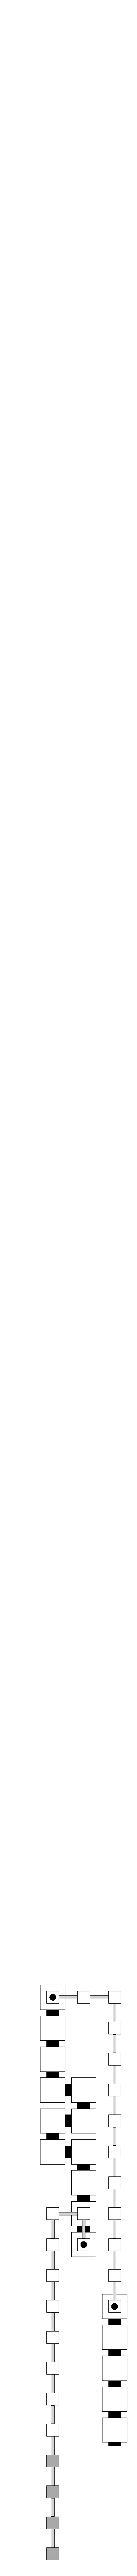
\includegraphics[width=0.2\textwidth]{digit_tops/digit_top_case3_msr}
            \caption{\label{fig:digit_top_general} General}
        \end{subfigure}%
        ~
        \begin{subfigure}[t]{0.2\textwidth}
            \centering
            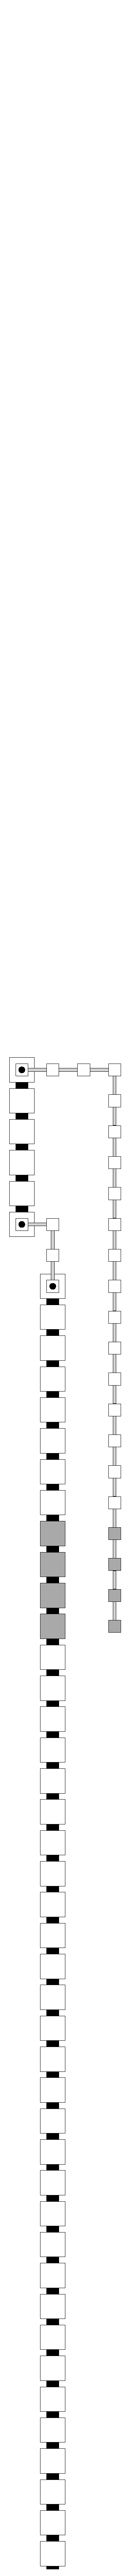
\includegraphics[width=0.2\textwidth]{digit_tops/digit_top_case2_digit2_msr}
            \caption{\label{fig:digit_top_case2_digit2_msr} Digit 2 -- Case 2}
        \end{subfigure}%
        ~
        \begin{subfigure}[t]{0.2\textwidth}
            \centering
            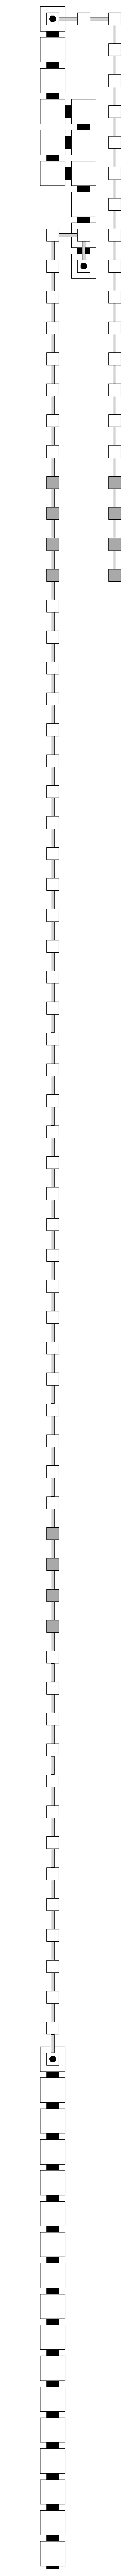
\includegraphics[width=0.2\textwidth]{digit_tops/digit_top_case1_digit1_msr}
            \caption{\label{fig:digit_top_case1_digit1_msr} Digit 1 -- Case 1}
        \end{subfigure}%
        ~
        \begin{subfigure}[t]{0.2\textwidth}
            \centering
            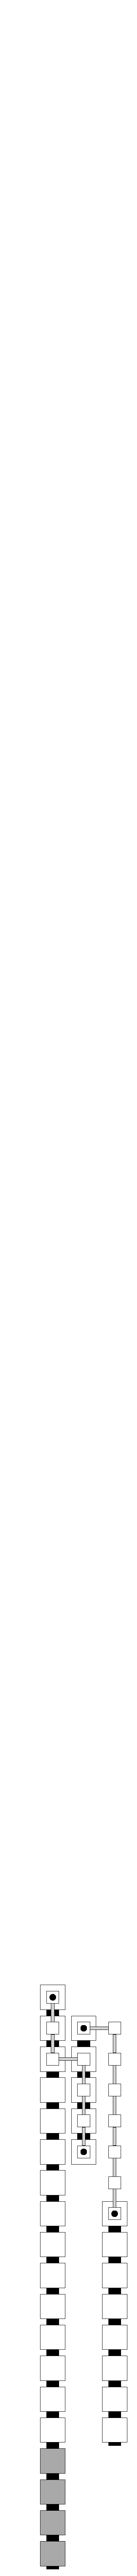
\includegraphics[width=0.2\textwidth]{digit_tops/digit_top_case2_digit1_msr}
            \caption{\label{fig:digit_top_case2_digit1_msr} Digit 1 -- Case 2}
        \end{subfigure}%
        ~
        \caption{\label{fig:digit_tops} {\tt Digit\_Top} gadgets}
    \end{figure}
\end{itemize}
\vspace{1cm}